Dynamic pricing is the canonical in-field reinforcement-learning problem for economics. Unlike simulator-based training, the agent learns from real customers, so \textit{exploration} is not an abstract sampling cost: a bad price loses revenue today and may affect the customer relationship. A seller faces $T$ customers in sequence, sets one price for each customer, and observes only whether the customer bought.\footnote{\citet{Rothschild1974} posed pricing under demand uncertainty as a two-armed bandit problem. His insight was that a \textit{myopic} seller can get stuck at a suboptimal price forever, because exploiting the currently best-looking price generates no information about alternatives.} The seller does not observe the customer's willingness to pay.

\textit{Regret}, the total revenue gap between the seller's policy and the best benchmark price or pricing rule, is the central measure. If the benchmark earns $r^*$ per customer, a policy with regret $R(T)$ earns $T r^* - R(T)$ in total. The central question is what economic structure turns pricing from a slow arm-learning problem into a fast demand-learning problem. With no useful structure, regret is polynomial in $T$. With enough structure, such as well-separated parametric demand, sparse contextual demand, revealed-preference bounds, or smooth monotone demand curves, learning can be much faster. But the assumptions matter, since an unknown noise distribution, strategic buyers, or fairness constraints can restore high regret even when the demand model looks rich.

\subsection{Foundations}
\label{sec:dp_foundations}

\subsubsection{No Structure on Demand}
\label{sec:kleinberg}

\citet{Kleinberg2003} study the benchmark case where the seller knows almost nothing. Customers arrive with valuations drawn i.i.d.\ from an unknown distribution on $[0,1]$, and the seller posts a price from a continuous set. The demand curve $D(p) = \Pr(v \geq p)$ is unknown; the only feedback is whether each customer bought. The seller's goal is to minimize regret against the single price $p^*$ that maximizes $p \cdot D(p)$. Kleinberg and Leighton prove that the minimax regret is $\Theta(\sqrt{T})$.\footnote{The upper bound, $O(\sqrt{T \log T})$, discretizes $[0,1]$ into $K = \lceil (T/\log T)^{1/4} \rceil$ prices and runs the UCB1 algorithm of \citet{auer2002}. The lower bound, $\Omega(\sqrt{T})$, constructs a family of demand curves parameterized by the location of the optimal price $p^* \in [0.3, 0.4]$. The key tension: posting prices far from $p^*$ is informative about demand but costly in revenue; posting prices near $p^*$ is cheap but uninformative. Resolving this tension costs at least $\Omega(\sqrt{T})$ in cumulative revenue. UCB1 \citep{auer2002} selects the price maximizing $\hat{\mu}_{p_k}(t) + \sqrt{2\ln t / N_{p_k}(t)}$, where $\hat{\mu}_{p_k}(t)$ is the empirical mean profit and $N_{p_k}(t)$ the number of trials; the second term is an exploration bonus that shrinks as a price is tried more, implementing the principle of optimism in the face of uncertainty.}

The rate is a useful baseline. After 10,000 customers, $\sqrt{T}$ regret is roughly 100 customers' worth of revenue lost to learning. No algorithm can improve on this worst-case rate without adding structure to $D$. For adversarial valuations, where a worst-case opponent rather than a fixed distribution chooses customer values, the minimax regret rises to $\Theta(T^{2/3})$, achieved by the Exp3 algorithm\footnote{\emph{Exp3} \citep{auer2002nonstochastic} maintains a weight $w_k(t)$ for each price, selecting $p_k$ with probability proportional to $w_k(t)$ and updating the chosen price's weight by $\exp(\eta \hat{r}_{k,t})$ where $\hat{r}_{k,t}$ is the revenue importance-weighted by the selection probability; because no model of demand is assumed, the guarantee holds against an adversary who chooses valuations after observing the algorithm.} on a discretized price grid. I focus on the stochastic setting throughout this chapter.

\subsubsection{Parametric Demand}
\label{sec:broder}

\citet{Broder2012} show that parametric demand is not automatically enough. Let $d(p; z) = \Pr(V \geq p)$, where $z \in \mathbb{R}^n$ is an unknown parameter governing the demand curve. The seller observes binary purchase decisions and updates a maximum likelihood estimate of $z$. Under standard regularity conditions (bounded demand, unique optimal price, smooth revenue function), the minimax regret is again $\Theta(\sqrt{T})$.\footnote{The lower bound (Theorem 3.1 of \citet{Broder2012}) constructs a linear demand family where all demand curves pass through the same point at the optimal price $p^*(z_0)$. Observing purchases at this price provides no information about $z$. An MLE-Cycle policy that interleaves dedicated exploration rounds with greedy pricing achieves the matching upper bound $O(\sqrt{T})$ (Theorem 3.6).} What matters is not whether the model has a finite-dimensional parameter, but whether profitable prices are also informative about that parameter.

The picture changes under a ``well-separated'' condition requiring that every price in the feasible set is informative about the demand parameter. Formally, the Fisher information $I(p, z)$ is bounded below by $c_f > 0$ for all prices $p$ and parameters $z$.\footnote{This means no two demand curves $d(p; z)$ and $d(p; z')$ cross on the pricing interval, so every purchase observation distinguishes the two hypotheses. In the lower-bound family of Theorem 3.1, the curves all cross at $p = 1$, which is why the $\sqrt{T}$ floor emerges.} Under well-separation, a pure greedy policy (MLE-Greedy, pricing at $p^*(\hat{z}_t)$ each period) achieves $O(\log T)$ regret (Theorem 4.8), because every price is informative and dedicated exploration rounds become unnecessary.

\begin{figure}[t]
\centering
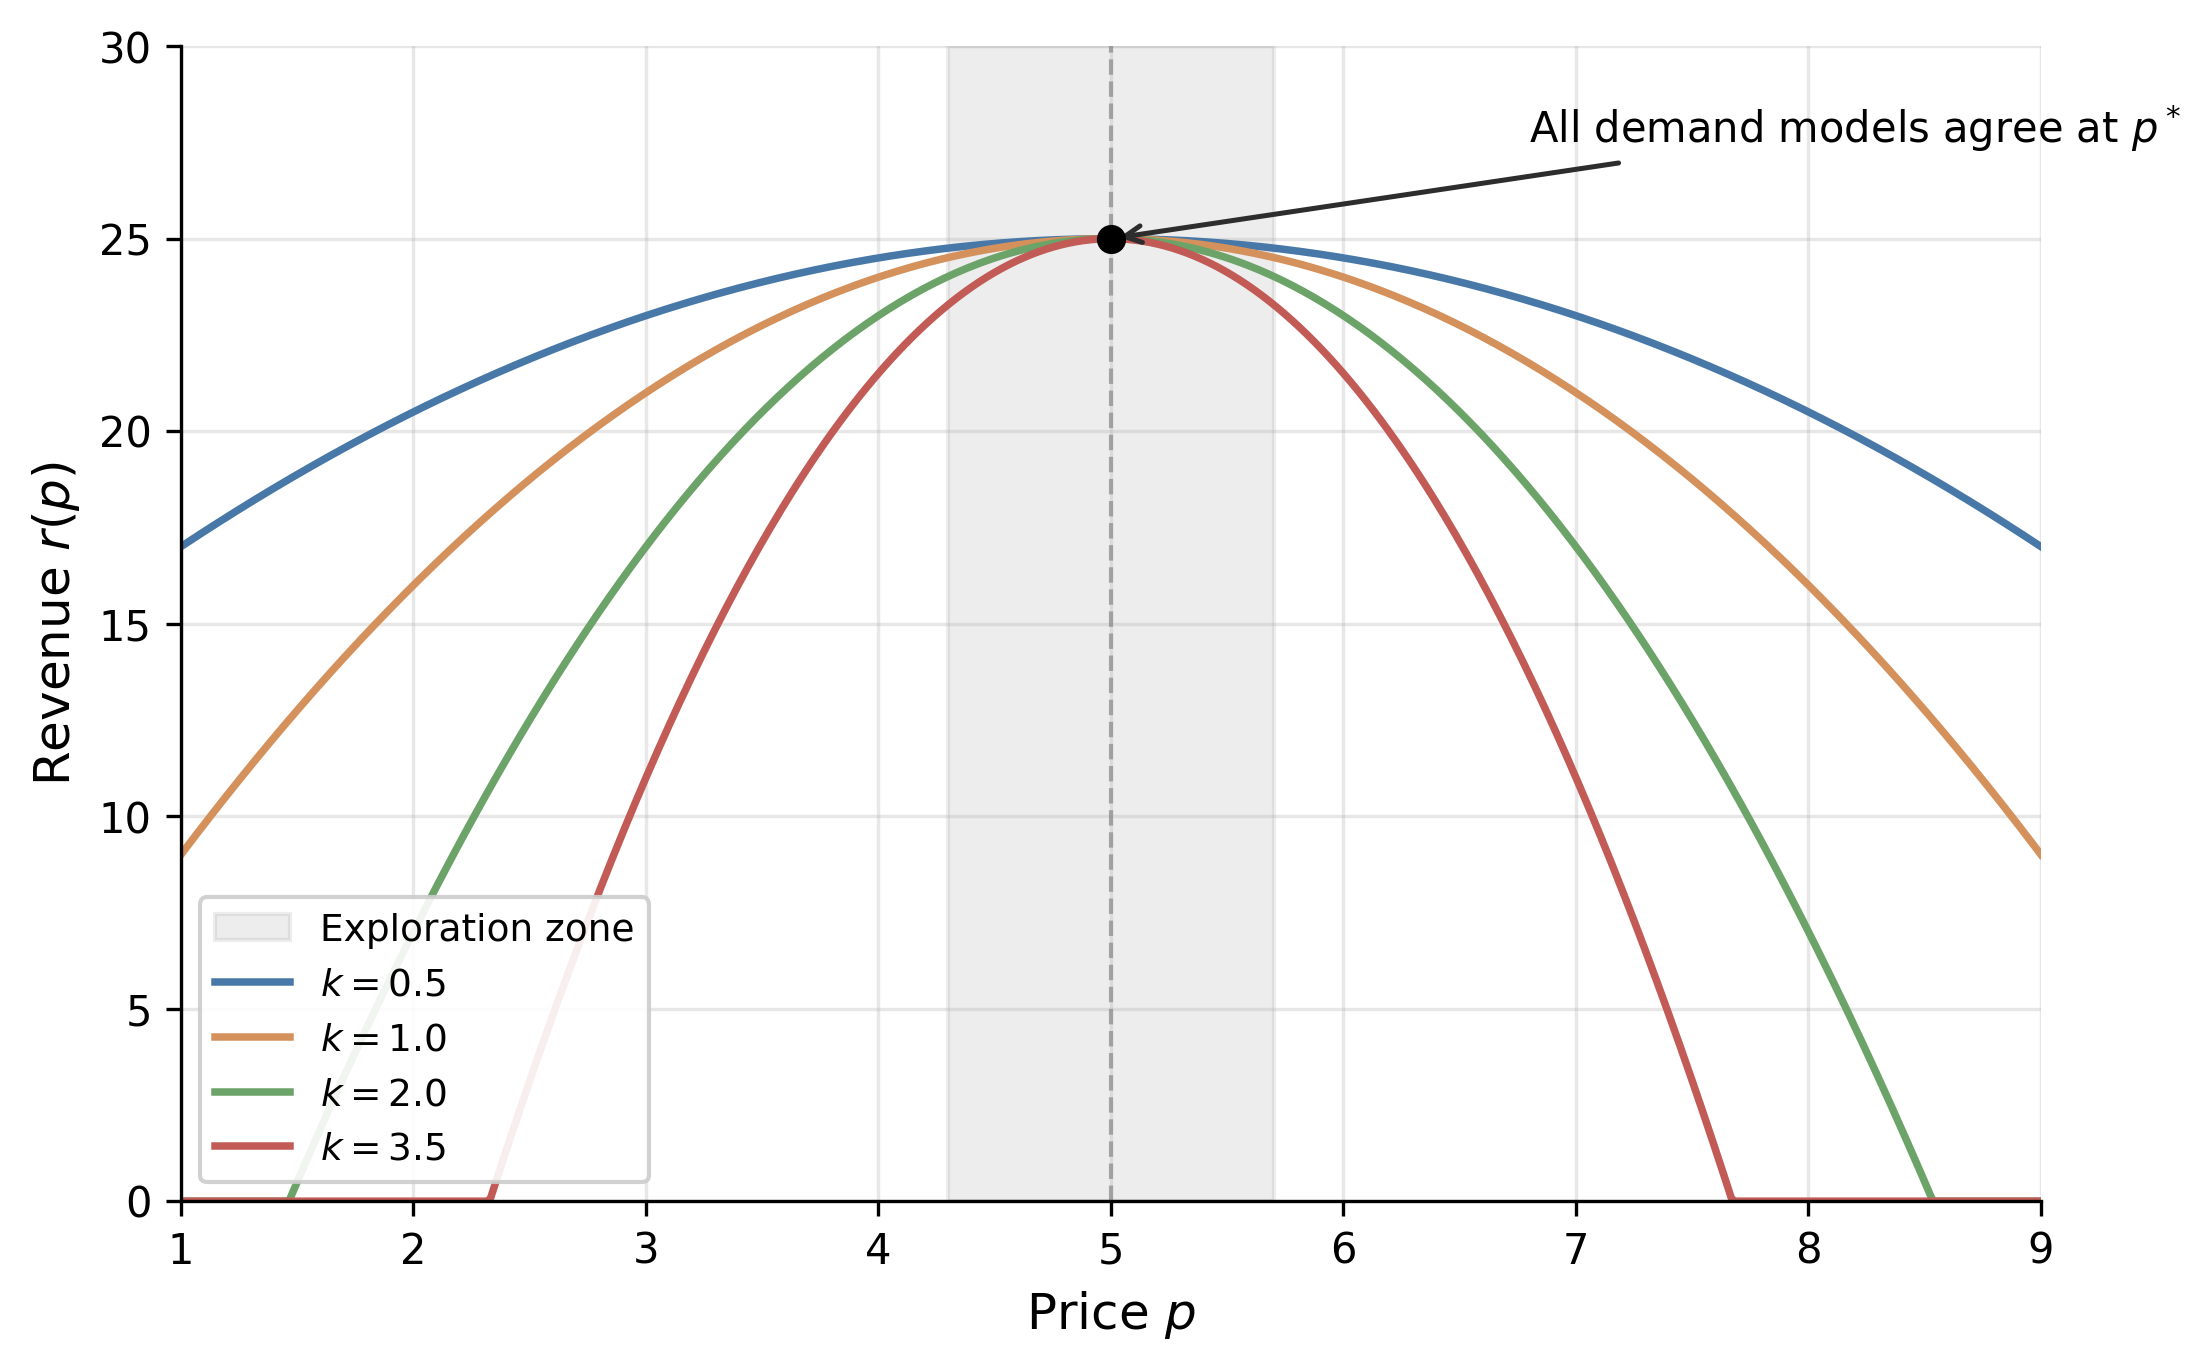
\includegraphics[width=0.7\textwidth]{../ch07_bandits/sims/uninformative_price.png}
\caption{Revenue curves $r(p) = r^* - k(p - p^*)^2$ for four demand curvatures $k \in \{0.5, 1.0, 2.0, 3.5\}$. All revenue curves share the maximizer $p^* = 5$; the underlying demand curves (not shown here, see \citet{Broder2012} Theorem 3.1) are linearly distinct but cross at $p^*$. Within the illustrative exploration window $|p - p^*| \leq 0.7$ (shaded; half-width is pedagogical, not derived), revenue separation across the four curves is at most $1.72$ units, about 7\% of $r^*$, which is small relative to typical purchase-noise variance at this scale.}
\label{fig:uninformative_price}
\end{figure}

\subsubsection{High-Dimensional Features with Sparsity}
\label{sec:javanmard}

\citet{Javanmard2019} extend the setting to products described by $d$-dimensional feature vectors $x_t$. The market value is $v_t = x_t^\top \theta_0 + z_t$, where $\theta_0 \in \mathbb{R}^d$ is unknown and $z_t$ is i.i.d.\ noise from a known log-concave distribution $F$.\footnote{Log-concavity of $F$ and $1 - F$ is satisfied by the normal, logistic, uniform, Laplace, and exponential distributions. It ensures that expected revenue $p \cdot [1 - F(p - x_t^\top \theta_0)]$ is strictly quasi-concave in $p$, giving a unique optimal price.} Only $s_0$ of the $d$ coordinates of $\theta_0$ are nonzero, but the seller does not know which ones.

Their RMLP algorithm (Regularized Maximum Likelihood Pricing) operates in episodes whose lengths double (1, 2, 4, 8, \ldots). At each episode boundary, the seller fits a LASSO-penalized maximum likelihood estimate of $\theta_0$ using data from the previous episode, then prices greedily throughout the current episode. The regret is $O(s_0 \log d \cdot \log T)$ (Theorem 4.1), with a matching lower bound of $\Omega(s_0 (\log d + \log T))$ (Theorem 5.1). The reason this beats $\sqrt{T}$ connects back to the Broder lower bound. In the parametric model of Section~\ref{sec:broder}, all demand curves can cross at the optimal price, making that price uninformative. Here, customer features vary across periods, so the aggregate demand function at any fixed price changes in proportion to the estimation error in $\theta_0$. Every price is informative, and dedicated exploration rounds become unnecessary.\footnote{If some feature directions are rarely observed, the seller cannot learn all coordinates of $\theta_0$ quickly, and regret degrades to $O(\sqrt{\log(d) \cdot T})$ (Theorem 4.2). If the noise distribution belongs to a known parametric family but its scale parameter is unknown, regret reverts to $\Omega(\sqrt{T})$ (Theorem 7.1), foreshadowing the result of \citet{Xu2021} discussed in Section~\ref{sec:xu}.} Even with hundreds of features, if only a handful matter, learning is fast.

\subsection{Revealed Preference and Partial Identification}
\label{sec:misra}

\subsubsection{WARP-Based Elimination}

\citet{Misra2019} bring economic theory into the bandit pricing framework. Their model has $K$ discrete prices, $S$ consumer segments (segment membership observed, but valuations unknown), and within-segment heterogeneity $\delta$. A consumer in segment $s$ has valuation $v_i = v_s + n_i$, where $v_s$ is the segment midpoint and $n_i \in [-\delta, \delta]$ is idiosyncratic noise. The key structural assumption is WARP (Weak Axiom of Revealed Preference): if a consumer buys at price $p$, she would buy at any lower price $p' < p$.

WARP turns a binary purchase into more information than a single arm reward. If a customer in segment $s$ buys at \$80, then prices below \$80 are also feasible for that customer; if she refuses \$120, prices above \$120 are also ruled out. Aggregating these inequalities gives partial identification of each segment's valuation. Suppose the seller has offered several prices to segment $s$. Define $p_s^{\min} = \max\{p_k : \text{all observed segment-$s$ customers bought at } p_k\}$ and $p_s^{\max} = \min\{p_k : \text{no observed segment-$s$ customer bought at } p_k\}$. Then the segment midpoint lies in $[p_s^{\min}, p_s^{\max}]$, and within-segment heterogeneity satisfies $\hat{\delta}_s \leq (p_s^{\max} - p_s^{\min})/2$. These bounds propagate to aggregate demand: for each price $p_k$, the seller constructs upper and lower bounds on total profit $\pi(p_k) = p_k \cdot D(p_k)$. When the profit upper bound at some price falls below the best profit lower bound across all prices, that price is dominated and permanently eliminated from consideration.

The UCB-PI algorithm combines dominance elimination with a price-scaled exploration bonus:
\begin{equation}
\label{eq:ucbpi}
I_{p_k}(t) = \hat{\mu}_{p_k}(t) + p_k \sqrt{\frac{2 \ln t}{N_{p_k}(t)}}
\end{equation}
if $p_k$ is not dominated, and $I_{p_k}(t) = 0$ otherwise, where $\hat{\mu}_{p_k}(t)$ is the average profit observed at price $p_k$ and $N_{p_k}(t)$ is the number of trials.\footnote{Standard UCB1 uses an exploration bonus of $\sqrt{2\ln t / N_{p_k}(t)}$, which assumes rewards in $[0,1]$. Since profit at price $p_k$ is bounded by $p_k$, scaling the bonus by $p_k$ tightens exploration for cheap prices that cannot contribute much profit regardless.} The improvement over standard UCB1 comes from two design choices. First, dominance elimination reduces the effective number of arms the algorithm must explore. Second, the $p_k$ scaling focuses exploration on prices where uncertainty actually matters for profit. These gains come from pruning dominated arms and calibrating arm-level exploration; they do not fully exploit smoothness or monotone dependence across nearby prices. Together, within the partial-identification model, these yield $O(\log T)$ regret.
\begin{equation}
\mathbb{E}[R_T(\text{UCB-PI})] \leq \sum_{k \neq k^*} \frac{8 p_k \log T}{\Delta_k} + \left(1 + \frac{\pi^2}{3}\right) \sum_{k=1}^K \Delta_k
\end{equation}
where $\Delta_k = \mu_{k^*} - \mu_k$ is the gap between arm $k$ and the optimal arm.\footnote{The first sum is the leading term, scaling as $O(\log T)$. The second sum is a constant that does not grow with $T$. Replacing $p_k$ with 1 recovers the standard UCB1 bound, which is looser.}

\citet{Misra2019} calibrate the model to an in-field deployment at ZipRecruiter, a B2B online recruiting platform. With 7,870 customers per month, 1,000 segments, and 10 price points from \$19 to \$399, UCB-PI achieves 98\% of oracle profit and produces 43\% higher profits during the first month of testing compared to a learn-then-earn alternative. The algorithm has both higher mean profit and lower variance, reflecting the value of eliminating dominated prices early.\footnote{For multi-product settings, \citet{Mueller2019} impose low-rank structure on the price-sensitivity matrix, achieving regret $O(T^{3/4}\sqrt{d})$ that scales with the latent demand dimension $d$ rather than the number of products. \citet{Badanidiyuru2013} extend the bandit framework to handle inventory constraints (``bandits with knapsacks''), relevant when the seller faces limited stock alongside the pricing decision.}

\subsubsection{Demand-Curve Learning}

\citet{Weaver2025} clarify what UCB-PI still fails to exploit. After dominated prices have been removed, the remaining prices are still learned mostly as separate arms. But pricing arms are not independent pulls; they lie on one demand curve. \citet{Misra2019} use revealed-preference bounds to eliminate dominated prices; \citet{Weaver2025} use smoothness and monotonicity to create informational externalities across prices.\footnote{For example, if demand at \$40 is estimated around 60\%, then a curve-learning bandit treats demand at \$41 as nearby rather than unknown from scratch; a monotone variant also rules out demand at \$41 being systematically higher than demand at \$40. Price scaling matters because the same five-percentage-point demand uncertainty creates \$0.50 of profit uncertainty at a \$10 price but \$5.00 at a \$100 price, so whether the optimal price is low, middle, or high on the grid changes the exploration problem.}

GP-UCB and GP-TS place a nonparametric prior on demand $D(p)$ rather than on each price's reward separately. An observation at one price therefore updates beliefs about nearby prices. The monotone variants add the economic restriction that demand weakly decreases with price by modeling both $D(p)$ and its derivative $D'(p)$ and constraining the derivative to be nonpositive. This is a stronger form of economic structure than arm elimination. It says not only which prices can be discarded but how evidence at one price should move beliefs about the rest of the price grid. That is why the incremental gains from partial identification can be small once a curve-learning bandit is already transferring information efficiently across prices.

\subsection{The Value of Knowing the Noise Distribution}
\label{sec:xu}

\citet{Xu2021} ask how much it helps to know the shape of demand uncertainty. In their model, a feature vector $x_t \in \mathbb{R}^d$ describes each sales session, the customer's valuation is $w_t = x_t^\top \theta^* + N_t$ where $\theta^*$ is unknown and $N_t$ is zero-mean i.i.d.\ noise with CDF $F$, and the seller observes only whether the customer bought at the posted price. The question is whether the seller knows $F$. The error distribution determines how purchase probabilities translate into valuations.\footnote{The regret benchmark here differs from Section~\ref{sec:kleinberg}. \citet{Kleinberg2003} and \citet{Broder2012} measure regret against the best fixed price; \citet{Xu2021} and \citet{Liu2024strategic} measure regret against the clairvoyant contextual policy that sets the optimal price $p_t^*$ for each customer's features $x_t$. The contextual benchmark is harder.}

If $F$ is known (the seller knows that demand shocks are, say, normally distributed with known variance), the EMLP algorithm (Epoch-based Maximum Likelihood Pricing) achieves regret $O(d \log T)$ (Theorem 3).\footnote{EMLP runs in doubling epochs of length $\tau_k = 2^{k-1}$. At each epoch boundary, the seller fits a maximum likelihood estimate $\hat{\theta}_k$ using data from the previous epoch, then prices greedily at $p_t = J(x_t^\top \hat{\theta}_k)$ throughout the epoch, where $J(u) = \arg\max_v \, v[1 - F(v - u)]$ is the revenue-maximizing price function. The key technical insight is that the negative log-likelihood is strongly convex (Lemma 7 of \citet{Xu2021}), so MLE concentrates at rate $O(d / \tau_k)$. Since regret is quadratic in the parameter estimation error (Lemma 5) and there are $O(\log T)$ epochs, the total regret is $O(d \log T)$.} After 10,000 customers with $d = 5$ features, the revenue loss is roughly 50 customers' worth, an improvement over the $\sqrt{T} \approx 100$ customers' worth that Kleinberg's lower bound imposes without structural knowledge.

If $F$ is unknown (even if only the variance of a Gaussian is unknown, with everything else known), the regret is at least $\Omega(\sqrt{T})$ (Theorem 12).\footnote{The lower bound constructs two noise variances $\sigma_1 = 1$ and $\sigma_2 = 1 - T^{-1/4}$. Any algorithm that performs well under both must spend $\Omega(\sqrt{T})$ revenue distinguishing the two cases. This extends the ``uninformative price'' phenomenon of \citet{Broder2012}: when the seller does not know $F$, there exist prices at which observed purchase behavior is nearly identical under different demand parameters.} The seller is back to the Kleinberg baseline: additional features alone do not buy logarithmic regret.

For fixed $d$, the gap between $O(d \log T)$ and $\Omega(\sqrt{T})$ grows like $\sqrt{T}/\log T$. This is not a constant-factor tuning issue; it is a change in the learning rate. When a modeler specifies a logit or probit demand model, the assumed noise distribution can buy logarithmic regret. Semiparametric approaches that leave the error distribution unspecified pay a concrete cost, reverting from logarithmic to polynomial regret.\footnote{\citet{Tullii2024} establish the tightest known bound under minimal distributional assumptions: if the noise distribution (c.d.f.) is merely Lipschitz continuous, the minimax regret is $\Theta(T^{2/3})$, strictly between the $\log T$ rate with known $F$ and the $\sqrt{T}$ rate with unknown $F$. \citet{Fan2024} consider a semiparametric setting where the noise density is smooth and connect the pricing problem to the econometrics of semiparametric estimation.}

\subsection{Strategic Buyers}
\label{sec:liu}

\citet{Liu2024strategic} introduce a different economic friction: buyers may respond strategically to the learning rule itself. At time $t$, a buyer arrives with true covariates $x_t^0 \in \mathbb{R}^d$ and valuation $v_t = \theta_0^\top x_t^0 + z_t$. The seller announces a pricing rule $p_t = g(\hat{\theta}_k^\top x_t)$, where $\hat{\theta}_k$ is the current parameter estimate. Crucially, the buyer observes this rule and can distort her reported features. She solves a cost-minimization problem:
\begin{equation}
\label{eq:manipulation}
\min_{\tilde{x}} \; (p - v_t) + \frac{1}{2}(\tilde{x} - x_t^0)^\top A (\tilde{x} - x_t^0)
\end{equation}
where $A$ is a positive definite matrix governing manipulation costs.\footnote{The matrix $A$ captures how costly it is for the buyer to distort each feature dimension. High eigenvalues of $A$ mean manipulation is expensive. This is the standard model of strategic classification \citep{Hardt2016}, adapted to pricing.} The first-order condition yields a systematic bias: the buyer shifts her features to make the seller's model predict a lower valuation, securing a lower price. The seller observes only the distorted features $\tilde{x}_t$, not the true $x_t^0$.

\begin{theorem}[Theorem 1 of \citet{Liu2024strategic}]
\label{thm:liu_impossibility}
Under standard regularity conditions, any pricing policy that treats reported features as truthful accumulates regret $\Omega(T)$.
\end{theorem}

Regret here is linear in $T$. Every standard dynamic pricing algorithm, including EMLP and RMLP, systematically underprices because it bases decisions on manipulated features, and the bias does not shrink with more data because the manipulation is endogenous to the pricing rule.

The fix is to jointly estimate demand parameters and manipulation behavior. \citet{Liu2024strategic} propose an episodic algorithm with two phases per episode. During the exploration phase, the seller posts uniform random prices that do not depend on features. Since the price is independent of $\tilde{x}_t$, buyers have no incentive to manipulate, and the seller observes true features $x_t^0$. During the exploitation phase, the seller uses the corrected pricing rule that anticipates the manipulation:
\begin{equation}
\label{eq:strategic_price}
p_t = g\left(\hat{\theta}_k^\top x_t + \hat{\beta}_k^\top A^{-1} \hat{\beta}_k \cdot g'(\hat{\theta}_k^\top x_t)\right)
\end{equation}
where $\hat{\beta}_k$ is the estimated coefficient on the manipulable features and $g$ is the optimal pricing function. This correction adds a markup that offsets the anticipated feature distortion.

\begin{theorem}[Theorem 2 of \citet{Liu2024strategic}]
\label{thm:liu_fix}
With known manipulation cost matrix $A$, the strategic pricing algorithm achieves regret $O(d\sqrt{T})$.
\end{theorem}

When $A$ is unknown, the seller can still recover $O(d\sqrt{T/\tau})$ regret by tracking repeat buyers across exploration and exploitation phases, where $\tau$ is the fraction of buyers who appear in both phases (Theorem 3). Higher repeat rates mean more matched pairs for estimating manipulation behavior.

A pricing rule changes buyer incentives, and those incentives change the data the seller sees. Incentive compatibility matters even in settings where the seller is ``just'' learning demand.\footnote{\citet{Agrawal2024ref} document a related phenomenon in pricing with reference effects. If consumers anchor on past prices, a static pricing policy that ignores reference dependence accumulates linear regret $\Omega(T)$.}

\subsection{Comparison of Regret Rates}
\label{sec:comparison}

Table~\ref{tab:regret_comparison} collects the regret rates discussed above. The dominant pattern is that stronger assumptions yield faster learning, but only when the assumptions make profitable actions informative about demand. For fixed dimension, the gap between $\log T$ and $\sqrt{T}$ grows without bound as $T \to \infty$, so the distinction is more than a constant factor. Strategic behavior is the outlier: it produces linear regret that no amount of data can overcome without explicit correction. Figure~\ref{fig:regret_rates} plots each rate on a log-log scale with all constants set to 1. The figure makes a qualitative asymptotic point; in practice the implicit constants in front of $\log T$ can dwarf those in front of $\sqrt{T}$ at modest horizons, so the visual ordering near $T = 10{,}000$ is illustrative rather than predictive of finite-sample behavior.

\begin{table}[!htbp]
\centering
\small
\caption{Regret rates in dynamic pricing under progressively stronger assumptions. $T$ is the number of customers, $d$ the feature dimension, $s_0$ the sparsity level. The last column translates asymptotic rates into concrete terms for $T = 10{,}000$ with $d = 5$, setting constants to 1.}
\label{tab:regret_comparison}
\resizebox{\textwidth}{!}{%
\begin{tabular}{@{}llllp{2.8cm}@{}}
\toprule
Paper & Demand & Noise & Regret & Per 10K ($d{=}5$) \\
\midrule
\citet{Kleinberg2003} & none & none & $\sqrt{T}$ & $\sim$100 lost \\
\citet{Broder2012} & parametric & known family & $\sqrt{T}$ & $\sim$100 lost \\
\citet{Broder2012} & param., well-sep. & known family & $\log T$ & $\sim$9 lost \\
\citet{Javanmard2019} & linear, $s_0$-sparse & known, log-conc. & $s_0 \log d \log T$ & fast if $s_0$ small \\
\citet{Xu2021} & linear, contextual & known & $d \log T$ & $\sim$46 lost \\
\citet{Xu2021} & linear, contextual & unknown var. & $\geq \sqrt{T}$ & $\sim$100 lost \\
\citet{Tullii2024} & linear, contextual & Lipschitz only & $T^{2/3}$ & $\sim$464 lost \\
\citet{Misra2019} & WARP & -- & $\log T$ & $\sim$9 lost \\
\citet{Liu2024strategic} & linear $+$ strategic & known, na\"ive & $T$ & never improves \\
\citet{Liu2024strategic} & linear $+$ strategic & known, corrected & $d\sqrt{T}$ & $\sim$500 lost \\
\bottomrule
\end{tabular}%
}
\end{table}

\begin{figure}[!htbp]
\centering
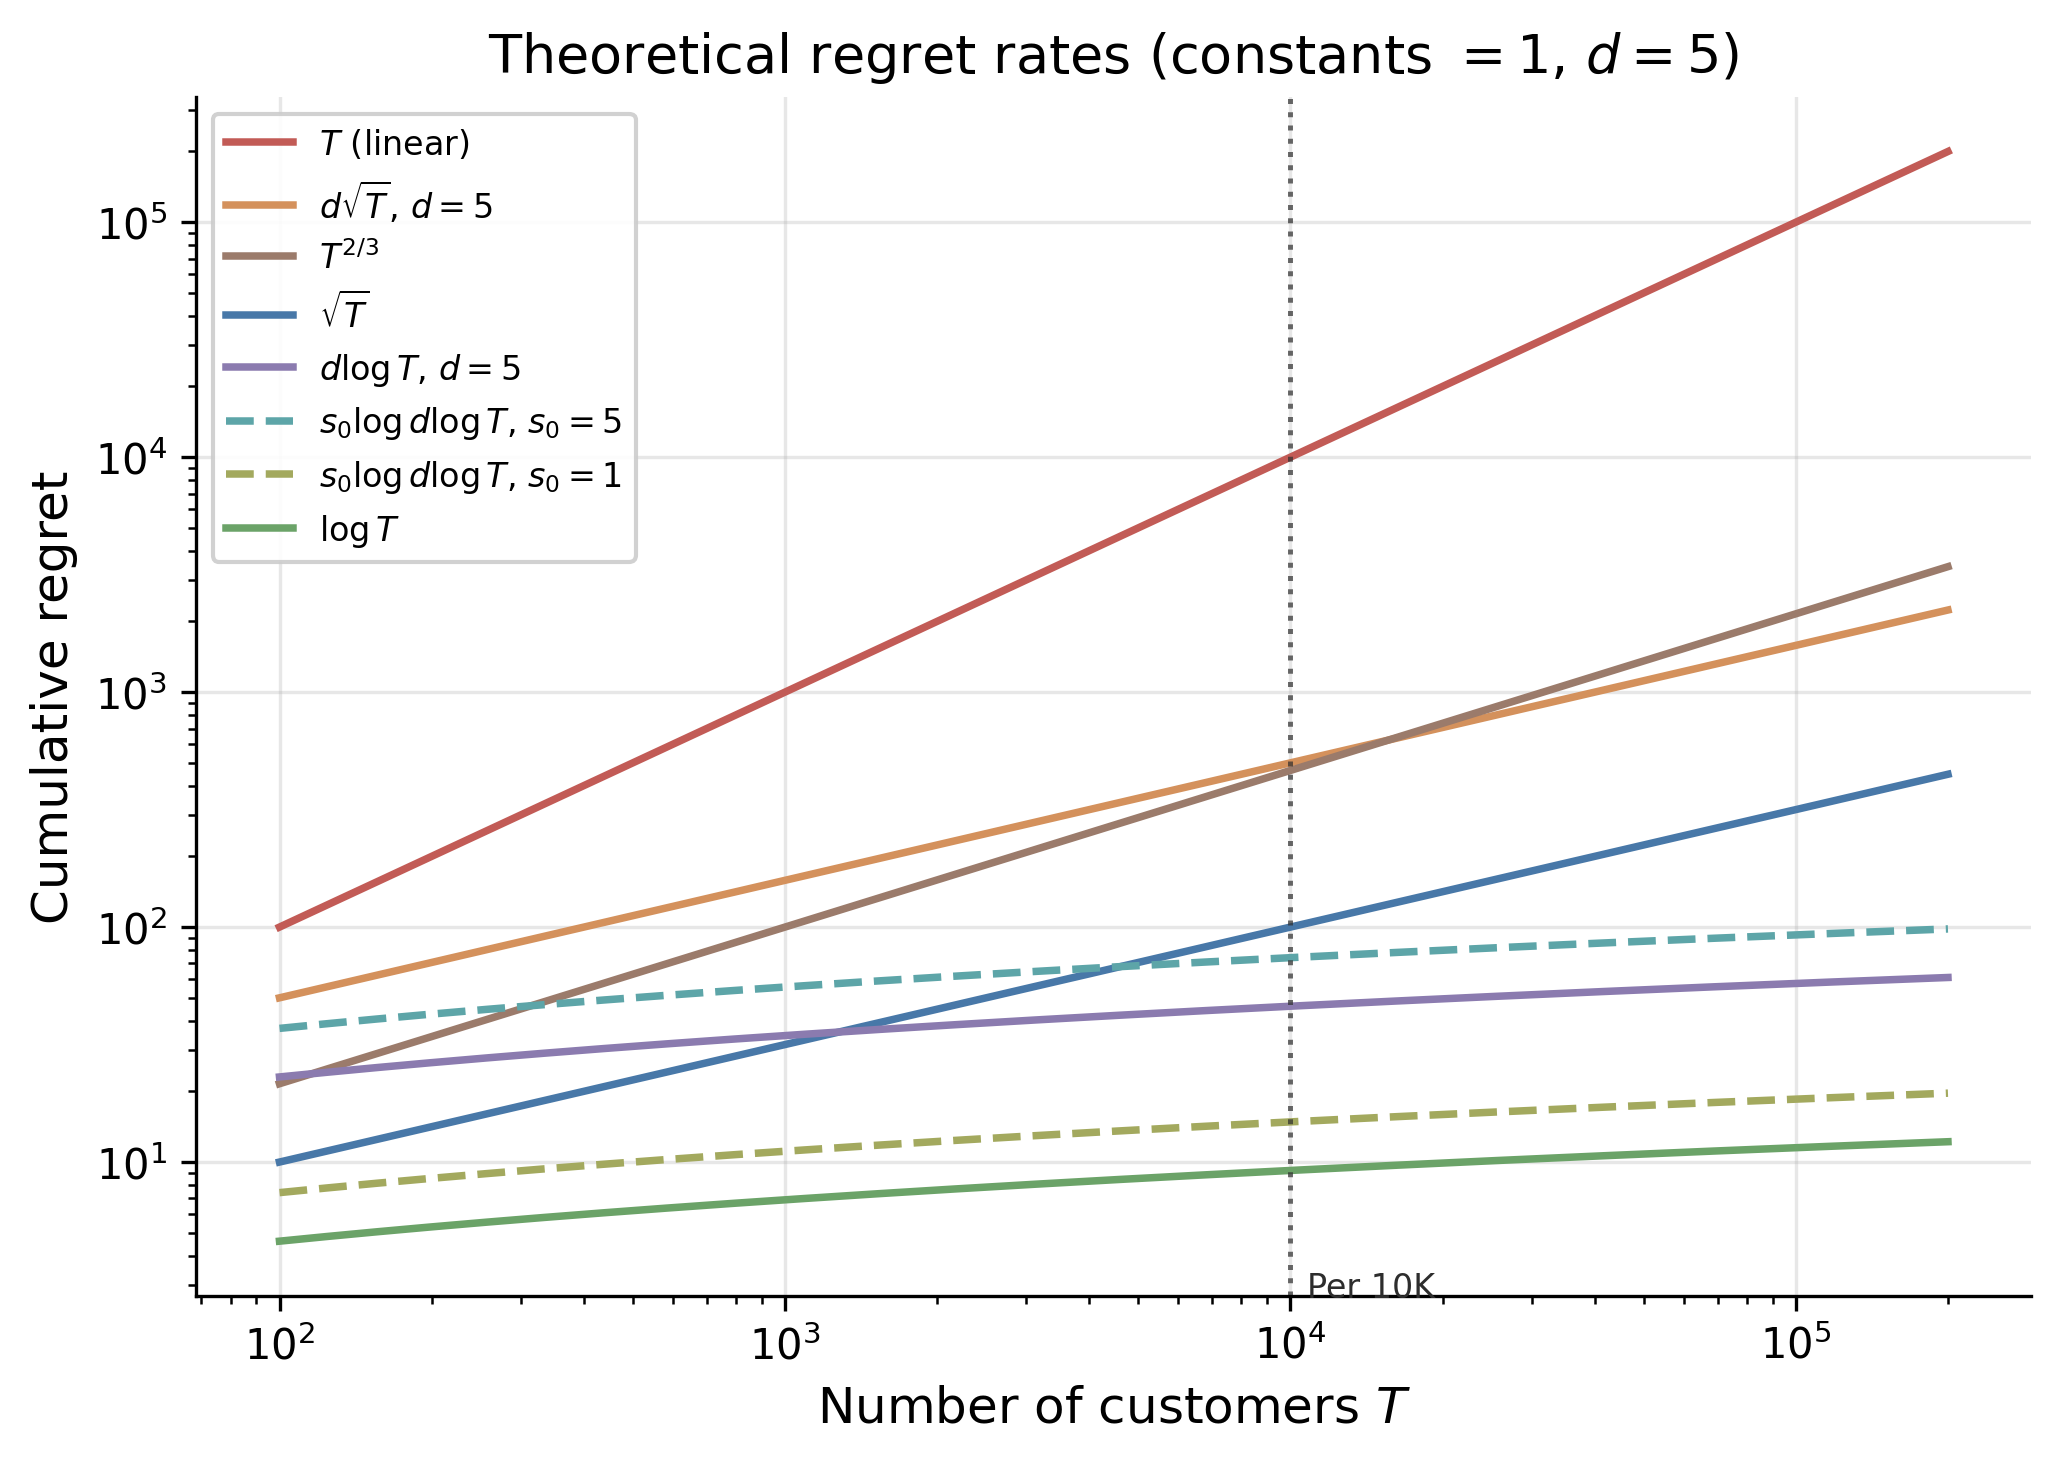
\includegraphics[width=0.75\textwidth]{../ch07_bandits/sims/regret_rates.png}
\caption{Theoretical regret rate functions at constants equal to 1, $d = 5$. Legend names the source paper for each rate. Two cases for the $s_0 \log d \log T$ rate are shown: $s_0 = 1$ (very sparse, $\approx 15$ lost at $T = 10{,}000$) and $s_0 = 5$ (here $s_0 = d$, $\approx 74$ lost), which at this constants-equal-to-1 calibration sits above $d \log T$ because $s_0 \log d \approx 8.0 > d = 5$; sparse dominates when $s_0 \ll d$. The vertical line marks $T = 10{,}000$, matching the ``Per 10K'' column of Table~\ref{tab:regret_comparison}.}
\label{fig:regret_rates}
\end{figure}

\subsection{Applications}
\label{sec:dp_applications}

This pattern extends beyond single-product posted pricing. Practical pricing systems are useful when they exploit structure that would be invisible to a generic bandit: low-rank substitution patterns across products, common elasticity parameters, capacity constraints, or shared demand forecasts.

\subsubsection{Joint Assortment and Pricing at Scale}

\citet{Cai2023} tackle the joint assortment-pricing problem, where a retailer must simultaneously choose which products to display and at what prices. With a large catalog and limited shelf space, the number of possible assortments is combinatorially vast; for a Chinese instant noodle producer with 176 products and 30 display slots, there are $\binom{176}{30} \approx 6.4 \times 10^{33}$ possible assortments before prices are even set. Customer demand also depends on market context such as region and season. In each period $t$, the retailer selects an assortment-pricing vector $a_t \in \mathbb{R}^{d_a}$ (encoding which products to display and at what prices), observes a context vector $x_t \in \mathbb{R}^{d_x}$ (encoding customer demographics and market conditions), and earns revenue $Y_t$. Cai et al.\ model expected revenue as $\mathbb{E}[Y_t \mid x_t, a_t] = a_t^\top \Theta^* x_t$, where $\Theta^* \in \mathbb{R}^{d_a \times d_x}$ is an unknown matrix assumed to have low rank $r \ll \min\{d_a, d_x\}$. The low-rank assumption is the demand-side analogue of factor models in asset pricing; a small number of latent dimensions (flavor preferences, seasonal effects, price sensitivity) explain most of the variation in purchasing behavior.

Their Hi-CCAB algorithm estimates $\Theta^*$ via penalized least squares, where the penalty is the nuclear norm (the sum of singular values) of $\Theta$. This penalty encourages low-rank solutions, playing the same role for matrices that the LASSO penalty plays for sparse vectors. The time-averaged regret is $\tilde{O}(T^{-1/6})$ with dimension dependence $r(d_a + d_x)$ rather than $d_a \cdot d_x$, so the effective parameter count scales with the number of latent factors, not the full product-by-context matrix. In simulation, Hi-CCAB achieves nearly four times the cumulative sales of the noodle producer's historical assortment strategies, averaged over 100 replications.

\citet{Ganti2018} deploy Thompson Sampling in-field for dynamic pricing at Walmart.com. Their MAX-REV-TS algorithm models demand for each item $i$ on day $t$ via a constant-elasticity function $d_{i,t}(p) = f_{i,t}(p/p_{i,t-1})^{\gamma_i^*}$, where $d_{i,t}(p)$ is unit sales at price $p$, $f_{i,t}$ is a baseline demand forecast at the previous day's price $p_{i,t-1}$, and $\gamma_i^* < -1$ is the unknown price elasticity. The structural assumption, that demand responds to price through a single elasticity parameter per item, reduces the learning problem from estimating a full demand curve to estimating one scalar per item. MAX-REV-TS places a Gaussian prior over the elasticity vector $\gamma^*$ and draws posterior samples at each period to solve a constrained revenue maximization problem. In a five-week in-field experiment on a basket of roughly 5,000 items, Thompson Sampling produced a statistically significant increase in per-item revenue relative to the passive pricing baseline.

\subsection{Simulation Study: Structural Knowledge and Curve Learning}
\label{sec:bandit_sim}

I use two simulations to make the chapter's taxonomy concrete. The first is a WARP and partial-identification ladder based on \citet{Misra2019}. The second is a Weaver-style curve-learning exercise that isolates the informational-externality point.

In the first simulation, I run six algorithms on the \citet{Misra2019} demand environment to trace how cumulative regret responds to increasing structural knowledge.\footnote{The environment has $K = 100$ prices on a grid from \$0.01 to \$1.00, $S = 1{,}000$ consumer segments with equal weights, within-segment heterogeneity $\delta = 0.1$, and segment midpoints $v_s \sim \mathrm{Uniform}(0.1, 0.9)$. A consumer purchases if and only if $v_i \geq p$ (WARP). Each algorithm runs across 10 seeds with $T = 200{,}000$ rounds.} This is a WARP and partial-identification demonstration, not a horse race against GP-UCB, GP-TS, or monotone GP demand-curve methods. The six algorithms, ordered by the structural knowledge they exploit, are: (0) $\varepsilon$-greedy with $\varepsilon = 0.1$, which never adapts its exploration rate; (1) Learn-Then-Earn (LTE), which explores uniformly for the first 5\% of rounds and then commits to the empirical best price; (2) UCB1 \citep{auer2002}, which adapts exploration via confidence bounds but ignores demand structure; (3) Thompson Sampling \citep{Thompson1933}, which maintains a Bayesian posterior over purchase rates\footnote{At each period the algorithm draws one sample $\tilde{\mu}_k$ from each arm's posterior over its purchase rate and selects the arm with the highest sampled expected profit $p_k \tilde{\mu}_k$; arms with uncertain posteriors have high-variance draws and are selected frequently, while well-estimated arms are selected in proportion to how likely they are optimal.}; (4) UCB-PI \citep{Misra2019}, which uses WARP to eliminate dominated prices and scales the exploration bonus by the price level\footnote{The UCB-PI implementation needs an estimate of the within-segment heterogeneity $\delta$. From the segments with both a strict lower and upper bound on the purchase threshold, I form per-segment half-widths $\hat{\delta}_s = (\hat{p}_{s,\max} - \hat{p}_{s,\min})/2$ and use $\hat{\delta} = \hat{\delta}_{\max} + (\hat{\delta}_{\max} - \overline{\hat{\delta}})$, which inflates the largest observed half-width by its gap from the mean. I am not aware of a published source for this exact form. It is included as a transparent reference point against the standard UCB-PI; \citet{Misra2019} estimates $\delta$ from the data but uses a different concrete expression.}; and (5) UCB-PI-tuned, which adds a variance-based refinement to the exploration bonus.

Within this WARP-only comparison, Table~\ref{tab:knowledge_ladder} reports cumulative regret at four checkpoints and Figure~\ref{fig:knowledge_ladder} shows the full trajectories. The finite-sample pattern is mixed. UCB-PI-tuned achieves the lowest regret by $T = 200{,}000$, but plain UCB-PI is worse than Thompson Sampling and LTE in this run; at this horizon the finite-sample ordering inverts the asymptotic rate order, with UCB-PI's logarithmic-rate algorithm dominated by TS empirically and by LTE despite LTE's nominal $T^{2/3}$ rate. Rate diagnostics computed from these checkpoints reinforce this caveat: across $T \in \{10\text{K}, 50\text{K}, 100\text{K}, 200\text{K}\}$, only Thompson Sampling's $R/\sqrt{T}$ is close to stable; $\varepsilon$-greedy's $R/T$ and LTE's $R/T^{2/3}$ drift downward, UCB1's $R/\sqrt{T}$ grows, and $R/\log T$ for plain UCB-PI quadruples. The right conclusion is narrower. WARP-based elimination helps relative to plain UCB1, but good finite-sample performance depends on the variance-tuned implementation, $T = 200{,}000$ is too short for the predicted rates to visibly settle for most of these algorithms, and these results do not compare against curve-learning GP methods.

\begin{table}[!htbp]
\centering
\caption{Cumulative regret at four checkpoints on the \citet{Misra2019} environment, mean over 10 seeds, with each algorithm's theoretical rate.}
\label{tab:knowledge_ladder}
\begin{tabular}{llrrrrl}
\toprule
Level & Algorithm & $T{=}10$K & $T{=}50$K & $T{=}100$K & $T{=}200$K & Rate \\
\midrule
0 & $\varepsilon$-greedy & 160 & 624 & 1,158 & 2,263 & $\Theta(T)$ \\
1 & LTE (5\%) & 1,005 & 1,165 & 1,363 & 1,771 & $O(T^{2/3})$ \\
2 & UCB1 & 719 & 2,609 & 4,263 & 6,734 & $O(\sqrt{KT})$ \\
3 & Thompson & 290 & 628 & 844 & 1,136 & $O(\sqrt{KT})$ \\
4 & UCB-PI & 789 & 2,266 & 3,244 & 4,503 & $O(\log T)$ \\
5 & UCB-PI-tuned & 338 & 541 & 640 & 780 & $O(\log T)$ \\
\bottomrule
\end{tabular}

\end{table}

\begin{figure}[!htbp]
\centering
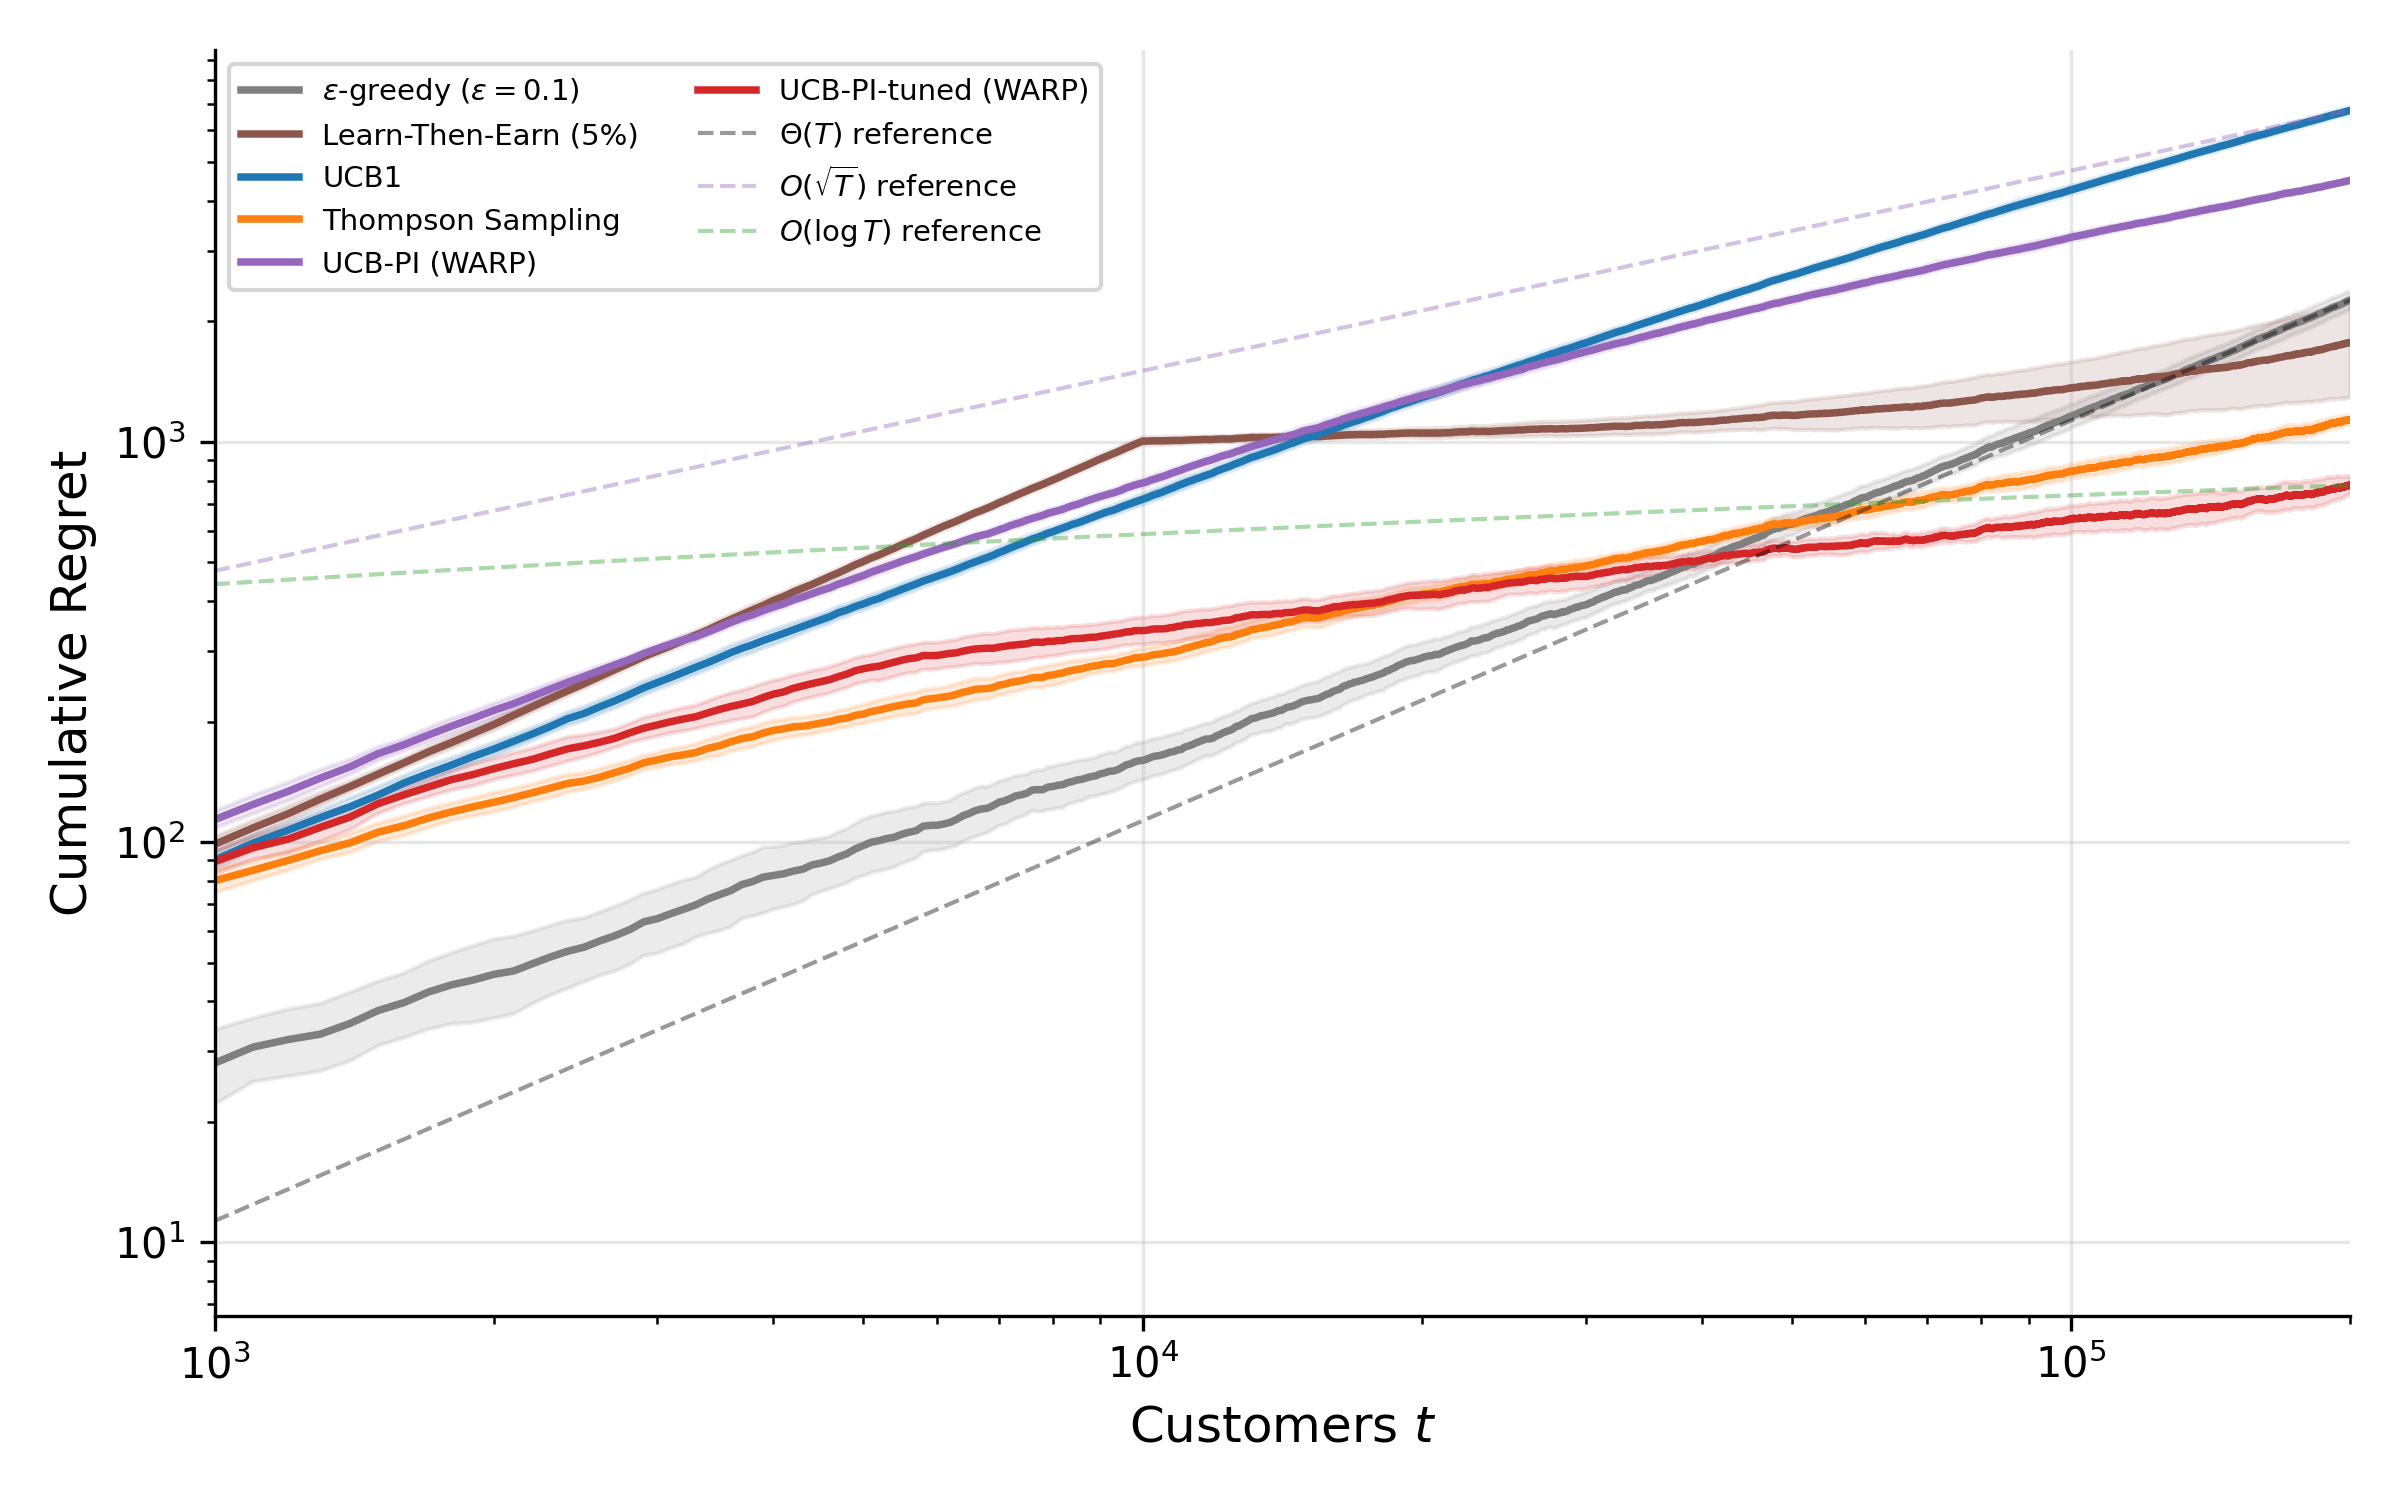
\includegraphics[width=0.7\textwidth]{../ch07_bandits/sims/knowledge_ladder_regret.png}
\caption{Cumulative regret on log-log axes ($K = 100$, $S = 1{,}000$, 10 seeds). Each algorithm's legend entry includes its theoretical regret rate. Dashed lines show $\Theta(T)$, $O(\sqrt{T})$, and $O(\log T)$ reference rates. Shaded regions are $\pm 2$ standard errors.}
\label{fig:knowledge_ladder}
\end{figure}

The second simulation makes the \citet{Weaver2025} critique operational. It is a small independent replication of the ten-price design in their simulations. Customer willingness to pay is drawn from $\mathrm{Beta}(2,9)$, $\mathrm{Beta}(2,2)$, or $\mathrm{Beta}(9,2)$, giving low-, middle-, and high-optimal-price cases. The tested prices are $p_a=a/10$ for $a=1,\ldots,10$, the firm updates prices every 10 customers, each run lasts $T=2{,}500$ customers, and the table averages over 1{,}000 simulation seeds. The algorithms are independent-arm Thompson Sampling, GP-UCB, GP-TS, GP-UCB-M, and GP-TS-M.\footnote{The GP code is an independent finite-grid implementation of the same demand-GP and derivative-sign ideas in \citet{Weaver2025}, not the authors' replication code. Demand, not reward, is the latent GP object. A batch sale rate is treated as a noisy demand observation with variance $0.25/n_a$. GP-UCB and GP-TS choose prices from posterior upper bounds or posterior draws of $D(p)$. The monotone variants form a joint RBF-GP over $D(0)$, $D(p)$, and $D'(p)$, enforce $D'(p) \leq 0$ through truncated-normal derivative draws, and reconstruct demand by integrating the derivative path on the price grid. GP-UCB-M uses upper quantiles of these constrained posterior curves.}\footnote{GP-UCB uses a constant exploration scale $\beta = 1.8$ rather than the growing schedule $\beta_t = 2\log(|\mathcal{X}|\, t^2 \pi^2 / (6\delta))$ of \citet{Srinivas2010}; the asymptotic regret rate changes only by a log factor, which is not separable from Monte Carlo noise at $T = 2{,}500$ averaged over 1{,}000 seeds. The GP prior mean $\mu_0(p) = 1 - p$ encodes a downward-sloping demand assumption, while independent-arm TS uses an uninformative $\mathrm{Beta}(1,1)$ prior; both methods adapt as data accumulates, and the reported gap is therefore between the worst-case (uniform-prior TS) and a best-case (shape-informed GP) Bayesian baseline.}

Figure~\ref{fig:curve_learning_pricing} plots cumulative profit as a percentage of the price-set oracle $\Pi_P^*$, and Table~\ref{tab:curve_learning_pricing} reports the final values. The low-optimal-price case is the clearest diagnostic. With $v \sim \mathrm{Beta}(2,9)$, Thompson Sampling earns 83.6\% of the grid oracle by $T=2{,}500$, while GP-TS-M earns 97.5\% and GP-UCB-M earns 98.3\%. In the middle case, TS reaches 93.5\% and the monotone GP variants reach about 97\%. In the high-price case, TS, GP-TS, and GP-UCB are already near oracle, while the monotone variants are slightly lower. The conclusion is therefore narrower and closer to \citet{Weaver2025}. Curve-level informational externalities are most valuable when independent-arm bandits are pulled toward high-price uncertainty even though the true optimum is low; when the optimal price is high, the same uncertainty is less damaging because the uncertain high-price region is also close to the profitable region.

\begin{figure}[!htbp]
\centering
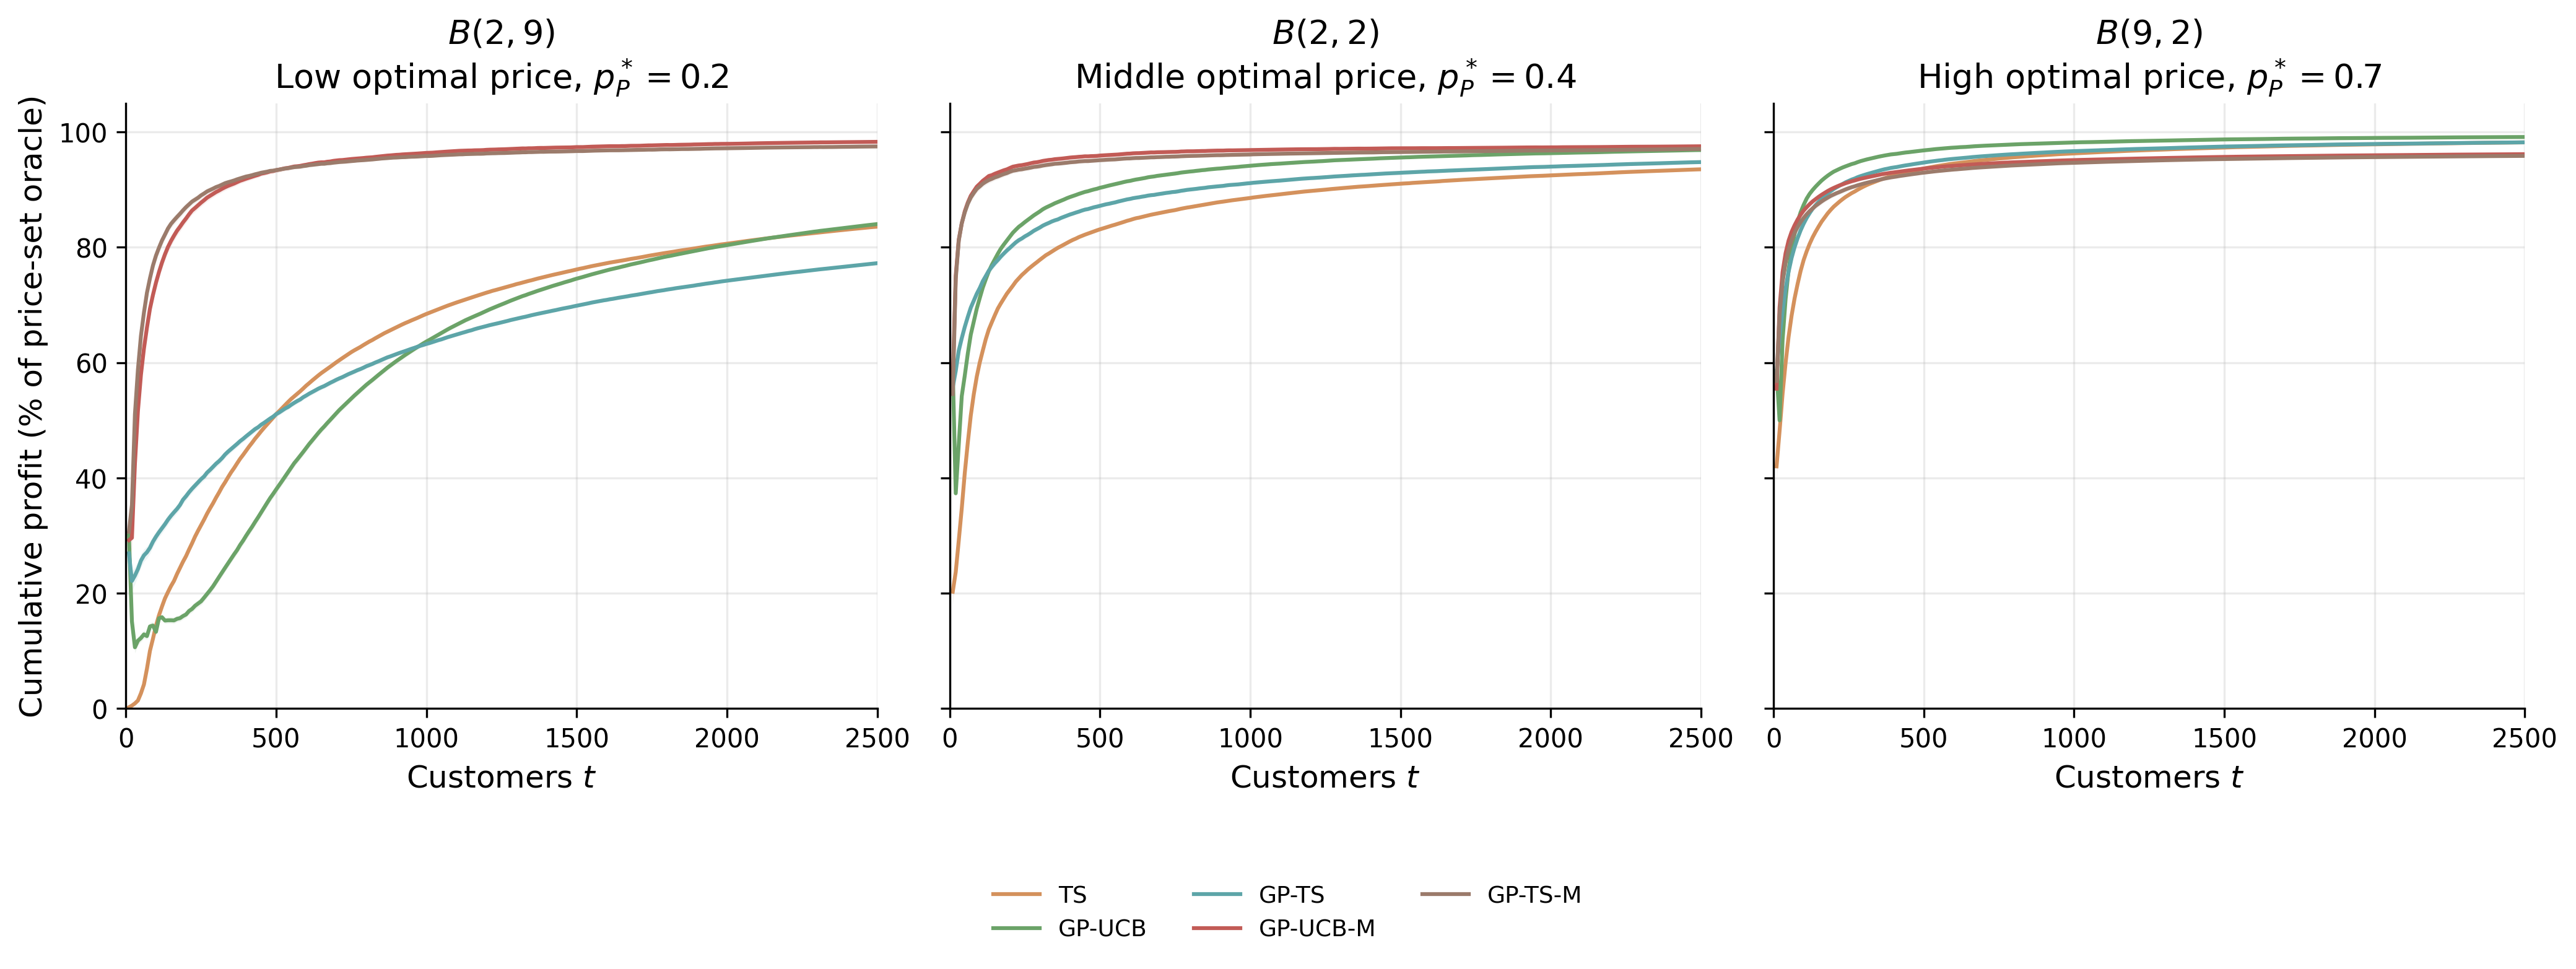
\includegraphics[width=\textwidth]{../ch07_bandits/sims/curve_learning_pricing_pct_oracle.png}
\caption{Weaver-style curve-learning pricing simulation across low, middle, and high optimal-price locations ($K = 10$, $T = 2{,}500$, 1{,}000 seeds, price updates every 10 customers). The $y$-axis is cumulative profit divided by the price-set oracle. GP-UCB and GP-TS share information across nearby prices; GP-UCB-M and GP-TS-M additionally impose $D'(p) \leq 0$ through derivative-constrained GP curves. Shaded regions are $\pm 2$ standard errors.}
\label{fig:curve_learning_pricing}
\end{figure}

\begin{table}[!htbp]
\centering
\begin{tabular}{lrrrrr}
\toprule
WTP & $p^*_P$ & TS & GP-TS & GP-TS-M & GP-UCB-M \\
\midrule
$B(2,9)$ & 0.2 & 83.6\% & 77.2\% & 97.5\% & 98.3\% \\
$B(2,2)$ & 0.4 & 93.5\% & 94.8\% & 97.0\% & 97.5\% \\
$B(9,2)$ & 0.7 & 98.2\% & 98.2\% & 95.8\% & 96.1\% \\
\bottomrule
\end{tabular}

\caption{Final cumulative profit as a percentage of the price-set oracle by $T=2{,}500$ in the Weaver-style curve-learning simulation.}
\label{tab:curve_learning_pricing}
\end{table}
